\section{Introduction}
The distributional hypothesis, the idea that the statistical distribution of linguistic items in context plays a key role in characterizing their semantic behavior \citep{harris:distributional, lenci:ds:models}, lies at the heart of modern word representation models. When trained on large enough data-sets, these models allow to project linguistic items into a unified vector space \citep{Liu2020}, producing distributional vectors commonly referred to as word embeddings.

A major distinction can be made between static and contextualized word embeddings. Static word vector representations obtained through models such as Word2Vec \citep{word2vec:mikolov2013} and fastText \citep{fasttext:bojanowski:2017} are context independent, that is to say a single word is always mapped to the same vector, irrespective of its context. On the other hand, in contextualized representations, produced by models such as BERT \citep{BERT:devlin2019}, each word vector is dependent on and embeds at least some information about its particular context of occurrence \citep{BERTology:rogers}.

The paper we examine \citep{garcia:acl} investigates whether and to what extent both static and contextualized embeddings are able to adequately represent different lexical-semantic relations, such as homonymy and synonymy. In other words, it evaluates whether such models can discriminate between unrelated meanings represented by the same word form (homonymy) and identify the same sense conveyed by different words (synonymy).

To this end the author compiles data-sets for four language varieties -- English, Spanish, Portuguese and Galician -- and carries out four experiments (see section \ref{sec:claims}). We manage to partially reproduce the original results and further test the author's hypotheses on a newly-compiled Italian data-set. Despite some discrepancies, our observations validate the claims of the original author.


\section{Scope of reproducibility}
\label{sec:claims}

For each language variety \citet{garcia:acl} carries out four experiments and reports the results in Table 4 of the original paper. We try to reproduce these results and in doing so to verify the hypothesis formulated for each of the four experiments.

\begin{itemize}
    \item \textbf{Experiment 1}: given a target-word and three identical words in different contexts, two of them synonyms of the target, we test whether the model correctly discriminates the outlier. As an example, consider rows 1.1 and 1.2 in Table \ref{table:triples-examples}. \textbf{Hypothesis}: static embeddings are expected to fail, producing three identical vectors, while contextualized models should correctly identify the outlier.

    \item \textbf{Experiment 2}: given a target-word and three different words in different contexts, two of them synonyms of the target, we test whether the model is biased towards one specific sense. For example, consider rows 2.1 and 2.2 in Table \ref{table:triples-examples}. The target-word \textit{coach} can either mean \textit{bus} or \textit{trainer}. If the model were biased towards the latter sense, it would always represent \textit{coach} closer to \textit{trainer} even in sentences where this would not make sense. \textbf{Hypothesis}: biased models will not identify the outlier sense. However, incorporating contextual information might be helpful.

    \item \textbf{Experiment 3}: given a target-word and three words in different contexts, two of them synonyms of the target, we test whether the model correctly discriminates the outlier. In this experiment the outlier is an homonym of one of the two synonyms. For example, consider rows 3.1 and 3.2 in Table \ref{table:triples-examples}. \textbf{Hypothesis}: static embeddings are likely to incorrectly represent homonyms closer than synonyms, while contextualized embeddings should model the three words correctly.

    \item \textbf{Experiment 4}: given a target-word and three different words, two of them synonyms of the target, we test whether the model correctly discriminates the outlier. In this experiment the outlier has to be in the same context as at least one of the two synonyms. As an example, consider rows 4.1 and 4.2 in Table \ref{table:triples-examples}. \textbf{Hypothesis}: static embeddings may pass the test as they tend to represent type-level synonyms closely. Contextualized models, on the other hand, might be puzzled at targets with different meanings occurring in the same context.
\end{itemize}


\section{Methodology}

\subsection{Datasets}
We work with the four data-sets provided by \citet{garcia:acl} and with an additional Italian data-set that we compiled ourselves. Each of the five data-sets is composed of triples, where each triple is characterized by a specific target-word and three sentences. Two of the sentences contain synonyms of the target-word or the target itself. The remaining sentence might contain either an homonym of the target, an homonym of one of the synonyms or an unrelated word. For each triple three features are given: \texttt{POS}, \texttt{Context} and \texttt{Overlap}.

The three features are obtained through a comparison between \texttt{Sent.1} and \texttt{Sent.2}, \texttt{Sent.1} and \texttt{Sent.3} as well as \texttt{Sent.2} and \texttt{Sent.3}. This allows to control for context, word and POS-tag overlap. As an example, consider row 4.2 in Table \ref{table:triples-examples}. For this triple the value of \texttt{Context} is \texttt{false|true|false}, as the first and last word occur in the same context, thus making the second comparison (\texttt{Sent.1} vs \texttt{Sent.3}) true. As another example, consider row 3.2. In this triple the value of \texttt{Overlap} is \texttt{false|false|true}, as the words in \texttt{Sent.2} and \texttt{Sent.3} share the same form. Lastly, looking at the same triple, the value of \texttt{POS} is \texttt{same|same|same}, as the three words are all nouns.

\begin{table*}[h]
    \centering
    \begin{tabularx}{\textwidth}{llXXX}
        \hline
        & \textbf{Target} & \textbf{Sent. 1} & \textbf{Sent. 2} & \textbf{Sent. 3} \\ \hline

        % examples sentence for exp. 1
        1.1 & Coach & He was appointed as the new \textbf{coach}. & She joined the team as \textbf{coach}. & We go to the airport by \textbf{coach}. \\ \hline
        1.2 & Match & He watched the football \textbf{match}. & Chelsea have a \textbf{match} with United. & He lit the \textbf{match} on his shoe. \\ \hline

        % examples sentence for exp. 2
        2.1 & Coach & We go to the airport by \textbf{coach}. & They traveled by \textbf{bus}. & She was appointed as the new \textbf{trainer}. \\ \hline
        2.2 & Bank & I used to work in a \textbf{bank}. & Banks are \textbf{financial institutions}. &  They camped on the \textbf{shores} of the lake. \\ \hline

        % examples sentence for exp. 3
        3.1 & Spring & We planted flowers in \textbf{spring}. & Cherry trees bloom in the \textbf{springtime}. & The \textbf{spring} in the fuel pump is broken. \\ \hline
        3.2 & Lead & They have an \textbf{advantage} of 28 points. & Before his goal, the team had the \textbf{lead}. & The detectives are chasing a new \textbf{lead}. \\ \hline

        % examples sentence for exp. 4
        4.1 & Drop & Temperatures \textbf{drop} to freezing at night. & Temperatures \textbf{fall} to freezing at night. & Temperatures \textbf{rise} to freezing at night. \\ \hline
        4.2 & Duck & I \textbf{duck} to dodge the ball. & She \textbf{lowers} her gaze. & I \textbf{raise} to dodge the ball. \\ \hline
    \end{tabularx}
\caption{Triples examples, two for each experiment. For each triple, two sentences contain words with the same meaning as the target, while the remaining one does not.}\label{table:triples-examples}
\end{table*}

The English, Spanish, Portuguese and Galician data-sets consist of 709, 645, 358 and 1365 triples, respectively. The Italian data-set is smaller and comprises 243 samples. Following \citet{garcia:acl}, we only consider triples containing words with the same POS-tag. We report the total number of such triples and their distribution per experiment in Table \ref{table:triples-distribution}.

% TABLE REPORTING ONLY TRIPLES WITH WORDS THAT HAVE THE SAME POS
\begin{table*}[ht]
    \centering
    \begin{tabularx}{\textwidth}{X|lllll}
        \hline
        \textbf{Language} & \textbf{E1} & \textbf{E2} & \textbf{E3} & \textbf{E4} & \textbf{Total} \\
        \hline
        Galician & 105 & 149 & 229 & 135 & 618 \\
        English & 52 & 58 & 91 & 68 & 269 \\
        Portuguese & 41 & 37 & 74 & 41 & 193 \\
        Spanish & 49 & 71 & 110 & 59 & 289 \\
        Italian & 59 & 80 & 54 & 50 & 243 \\
    \end{tabularx}
\caption{Total number of triples in which the \texttt{POS} feature is \texttt{same|same|same} together with their distribution per experiment.}\label{table:triples-distribution}
\end{table*}


\subsection{Model descriptions}
We work with two types of models, BERT monolingual and fastText. BERT models are loaded through the Transformers library \citep{transformers}. For English, we rely on the base-uncased BERT model by \citet{BERT:devlin2019}. For Portuguese and Spanish we use the base-cased models released by \citet{bertimbau} and \citet{beto}, respectively. For Galician, we rely on the small-cased model trained by the original author while for Italian we use the base-cased model originally provided by \citet{bertita}.

For fastText we use models of 300 dimensions and experiment with three architectures: skip-gram \citep{fasttext:bojanowski:2017}, CBOW \citep{fasttext:2018} and MCBOW, a variation of the latter \citep{fasttext:mcbow:2018}. Specifically, for English we work both with the official MCBOW\footnote{English MCBOW fastText: \url{https://dl.fbaipublicfiles.com/fasttext/vectors-english/wiki-news-300d-1M.vec.zip}} and skip-gram\footnote{English skip-gram fastText: \url{https://dl.fbaipublicfiles.com/fasttext/vectors-wiki/wiki.en.vec}} versions. For Spanish we use both the official skip-gram\footnote{Spanish skip-gram fastText: \url{https://dl.fbaipublicfiles.com/fasttext/vectors-wiki/wiki.es.vec}} and CBOW\footnote{Spanish CBOW fastText: \url{https://dl.fbaipublicfiles.com/fasttext/vectors-crawl/cc.es.300.vec.gz}} models. For Portuguese we rely on the skip-gram\footnote{Portuguese skip-gram fastText: \url{http://143.107.183.175:22980/download.php?file=embeddings/fasttext/skip_s300.zip}} version by \citet{fasttext:portuguese}. For Galician we use the skip-gram\footnote{Galician skip-gram fastText: \url{https://zenodo.org/record/4481614/files/fasttext_sg_300d_w5.zip?download=1}} model trained by \citet{garcia:acl} and for Italian the official skip-gram\footnote{Italian skip-gram fastText: \url{https://dl.fbaipublicfiles.com/fasttext/vectors-wiki/wiki.it.vec}} version.

\subsection{Experimental setup and code}
The four experiments described in section \ref{sec:claims} rely on BERT and fastText embeddings. For both architectures a number embedding creation strategies are explored. We only describe those for which a result is reported in Table 4 of the original paper. Note that whenever a word consists of more than one token (e.g. \textit{financial institutions}) the average of the token embeddings is considered.

For BERT models the following three approaches are tested:
\begin{itemize}
    \item \textbf{Sentence vector (\textit{Sent})}: an embedding obtained by averaging the representations of all the words in a given sentence, but the \texttt{[CLS]} and \texttt{[SEP]} tokens. Each representation is obtained by concatenating the vectors produced in the last four layers of the model.

    \item \textbf{Word vector sum (\textit{Add})}: an embedding of a specific word obtained by summing its representations across the last four layers of the model.

    \item \textbf{Word vector concatenation (\textit{Cat})}: an embedding of a specific word obtained by concatenating its representations across the last four layers of the model.

\end{itemize}

For fastText models the following three approaches are tested:
\begin{itemize}
    \item \textbf{Word vector (\textit{WV})}: an embedding of a specific word.

    \item \textbf{Sentence vector (\textit{Sent})}: an embedding obtained by averaging the representations of all the words in a given sentence.

    \item \textbf{Syntax (\textit{Syn3})}: an embedding of a specific word obtained by adding the word representation to those of its syntactic head and dependents. The underlying assumption is that the syntactic context of a word would characterize its meaning. Generating this embedding requires converting each sentence in each triple to a CoNLL-U format.

\end{itemize}

The output of each model is evaluated as follows: for each triple, where two words (\textit{a} and \textit{b}) are synonyms and a third one (\textit{c}) has a different meaning, three cosine similarities between their embeddings are computed: \textit{sim1} $=$ \texttt{cos(a, b)}, \textit{sim2} $=$ \texttt{cos(a, c)} and \textit{sim3} $=$ \texttt{cos(b, c)}. Ultimately, the model should be able to discriminate the outlier \textit{c} i.e. the output for a specific triple is correct only if \textit{sim1} $>$ \textit{sim2} and \textit{sim1} $>$ \textit{sim3}.

For each model and embedding creation strategy we compute four accuracy scores, one per experiment, and provide macro- and micro-average results across them. Lastly, for each embedding creation strategy, we also report the micro-average accuracy score across the entire set of generated embeddings. It is worth noting that for each language variety the corresponding data-sets also contain triples of sentences that are not part of any of the four experiments described in Section \ref{sec:claims}.

We only report results for triples in which the synonyms and homonyms belong to the same word category (\texttt{POS} $=$ \texttt{same|same|same}). This allows to focus on the semantic knowledge encoded in their embeddings rather than on the morpho-syntactic information.

We rely on the code-base released by the original author, modifying it where necessary and integrating it with a few additional scripts for statistics computation and data preparation.

\subsection{Computational requirements}
We work with pre-trained BERT and fastText models, relying on a 3.10GHz Intel Core i9-7940X CPU. The total running-time for the experiment is about 30 minutes.

\section{Results}
\label{sec:results}

\subsection{Results reproducing the original paper}
Our results partially match those reported in the original study. In particular, we successfully reproduce the accuracy scores for the Galician BERT and fastText models, as well as for the English BERT and Portuguese fastText ones. However, we also observe a number of discrepancies across English, Spanish and Portuguese. We plot the difference between our results and the original ones in Figure \ref{fig:acc-diff} and report the exact values in Table \ref{table:full-results} in the Appendix. Galician results are not included as they match the original ones but we provide them in our GitHub repository.

Looking at BERT, the scores we obtain for Portuguese and Spanish are mostly higher than those originally indicated, with only two exceptions for Spanish in experiment 2 (BERT sent) and experiment 4 (BERT add). Turning to fastText, the results for the English and Spanish skip-gram models also deviate from the original ones. Nonetheless, relying on the MCBOW \citep{fasttext:mcbow:2018} and CBOW \citep{fasttext:2018} implementations we manage to reproduce the original English and Spanish scores, respectively (see Table \ref{table:full-results}).

Overall, BERT models perform consistently better than fastText in the first three experiments across all languages, while fastText models score higher accuracy values in the fourth one.

% These plots represent the accuracy score difference between the results obtained from the reproduction
% study and those reported in the original paper i.e. (repro_result - original_result) = points on the plot 

\begin{figure}[ht]
\centering
\usepgfplotslibrary{groupplots}
\usetikzlibrary{positioning}

\pgfplotsset{every axis title/.append style={at={(0.9,0.7)}, fill=white}}

% define name and style for each model being plotted
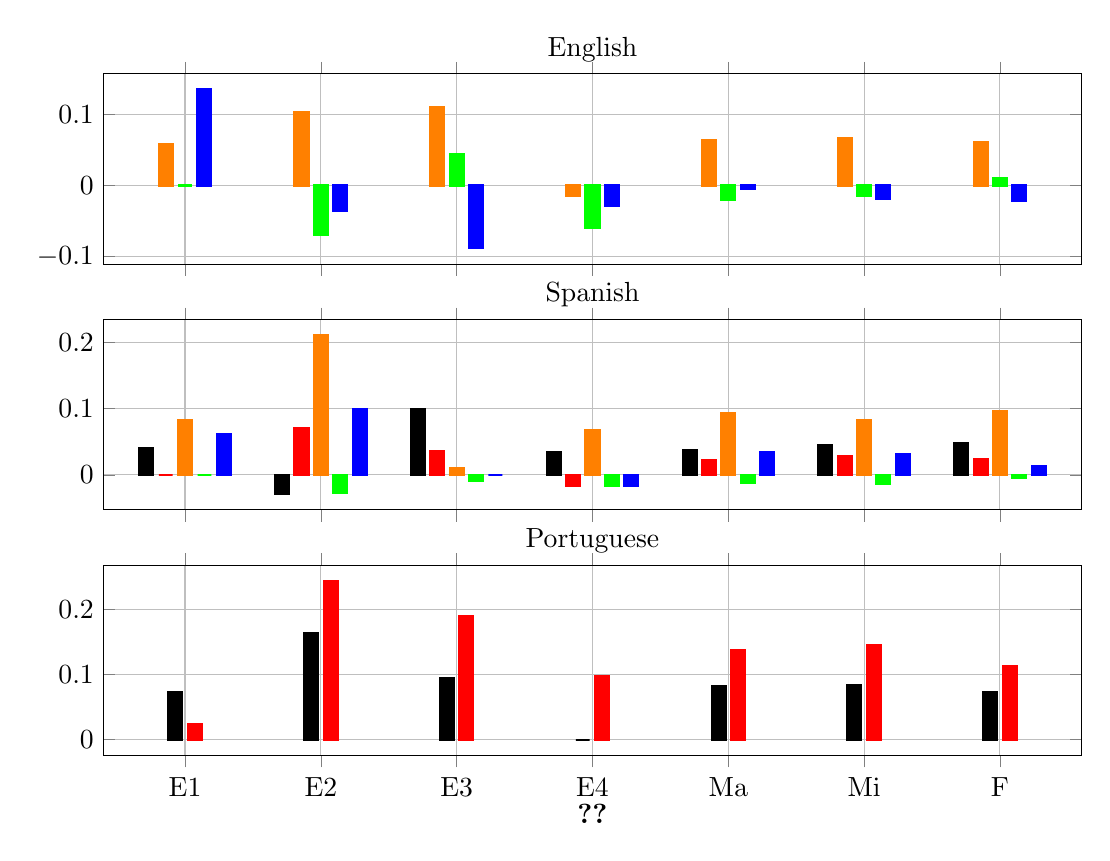
\begin{tikzpicture}[
    skipsent/.style={bar width=5pt, orange,fill=orange, thick},
    skipwv/.style={bar width=5pt, green,fill=green, thick},
    skipsyn3/.style={bar width=5pt, blue,fill=blue, thick},
    bertsent/.style={bar width=5pt, black,fill=black, thick},
    bertadd/.style={bar width=5pt, red,fill=red, thick}
]
\begin{groupplot}[
    group style={
        group name=results,
        group size=1 by 3,
        xlabels at=edge bottom,
        xticklabels at=edge bottom,
        % sets the space between the plots
        vertical sep=20pt
    },
    height=4cm,
    width=14cm,
    symbolic x coords={E1, E2, E3, E4, Ma, Mi, F},
    xtick={E1, E2, E3, E4, Ma, Mi, F},
    grid,
    ybar,
]

% ENGLISH RESULTS
\nextgroupplot
    \addplot[skipsent, ybar]
        % English fastText skip. sent: difference between Sent repro. and Sent orig. results
        coordinates {(E1, 0.058) (E2, 0.103) (E3, 0.11) (E4, -0.015)
                    (Ma, 0.064) (Mi, 0.067) (F, 0.061)};
    \addplot[skipwv, ybar]
        % English fastText skip. WV: difference between WV repro. and WV orig. results
        coordinates {(E1, 0.0) (E2, -0.069) (E3, 0.044) (E4, -0.059)
                    (Ma, -0.02) (Mi, -0.015) (F, 0.01)};
    \addplot[skipsyn3, ybar]
        % English fastText skip. Syn3: difference between Syn3 repro. and Syn3 orig. results
        coordinates {(E1, 0.135) (E2, -0.035) (E3, -0.088) (E4, -0.029)
                    (Ma, -0.004) (Mi, -0.019) (F, -0.021)};

% SPANISH RESULTS
\nextgroupplot[legend to name={CommonLegend},legend style={legend columns=5}]
    \addplot[bertsent]
        % Spanish BERT sent: difference between Sent repro. and Sent orig. results
        coordinates {(E1, 0.041) (E2, -0.029) (E3, 0.1) (E4, 0.034)
                    (Ma, 0.037) (Mi, 0.045) (F, 0.048)};
        \addlegendentry{BERT sent}

    \addplot[bertadd]
        % Spanish BERT add: difference between Add repro. and Add orig. results
        coordinates {(E1, 0.0) (E2, 0.071) (E3, 0.036) (E4, -0.017)
                    (Ma, 0.022) (Mi, 0.028) (F, 0.024)};
        \addlegendentry{BERT add}

    \addplot[skipsent]
        % Spanish fastText skip. sent: difference between Sent repro. and Sent orig. results
        coordinates {(E1, 0.082) (E2, 0.211) (E3, 0.01) (E4, 0.068)
                    (Ma, 0.093) (Mi, 0.083) (F, 0.097)};
        \addlegendentry{skip sent}
    
    \addplot[skipwv]
        % Spanish fastText skip. WV: difference between WV repro. and WV orig. results
        coordinates {(E1, 0.0) (E2, -0.028) (E3, -0.009) (E4, -0.017)
                    (Ma, -0.013) (Mi, -0.014) (F, -0.005)};
        \addlegendentry{skip wv}

    \addplot[skipsyn3]
        % Spanish fastText skip. Syn3: difference between Syn(3) repro. and Syn(3) orig. results
        coordinates {(E1, 0.062) (E2, 0.099) (E3, 0.0) (E4, -0.017)
                    (Ma, 0.035) (Mi, 0.031) (F, 0.013)};
        \addlegendentry{skip syn3}

% PORTUGUESE RESULTS
\nextgroupplot
    \addplot[bertsent]
        % Portuguese BERT sent: difference between Sent repro. and Sent orig. results
        coordinates {(E1, 0.073) (E2, 0.163) (E3, 0.095) (E4, 0.0)
                    (Ma, 0.082) (Mi, 0.083) (F, 0.073)};
    \addplot[bertadd]
        % Portuguese BERT add: difference between Add repro. and Add orig. results
        coordinates {(E1, 0.024) (E2, 0.243) (E3, 0.19) (E4, 0.097)
                    (Ma, 0.138) (Mi, 0.145) (F, 0.112)};

\end{groupplot}

% place title above each plot
\node[above = 0.03cm of results c1r1.north] {English};
\node[above = 0.03cm of results c1r2.north] {Spanish};
\node[above = 0.03cm of results c1r3.north] {Portuguese};

% place legend below last plot
\node[below = 0.5cm of results c1r3.south] {\ref*{CommonLegend}};

\end{tikzpicture}

\caption{\label{fig:acc-diff}Difference between our accuracy scores and those reported in the original paper computed across the four experiments, as well as for the macro (Ma), micro (Mi) and full (F) accuracy. For each language, only the models for which a discrepancy is observed are considered.
}

\end{figure}


\subsection{Results beyond the original paper}
We summarize our findings for the Italian data-set in Table \ref{table:results-ita}. Overall, the trend across the four experiments is consistent with the one we observe for the original language varieties, with BERT achieving the highest accuracy in the first three experiments for at least one embedding type (Vec) and fastText being the top performer in the last experiment. It is worth noting that the micro-average results across the four experiments (Mi) and the micro-average values on the whole data-set (F) are the same for each embedding type.

% TABLE REPORTING ITALIAN RESULTS
\begin{table*}[h]
    \centering
    \begin{tabularx}{\textwidth}{Xl|lllllll}
        \hline
        \textbf{Model}  &   \textbf{Vec}   &   \textbf{E1} &   \textbf{E2} &   \textbf{E3} &   \textbf{E4} &   \textbf{Ma} &   \textbf{Mi} &   \textbf{F}  \\
        \hline
        \multirow{3}{*}{\textbf{BERT}}   & Sent  &   0.763   &   0.8   &   0.741   &   0.14    &   0.611   &   0.642   &   0.642   \\
                                & Add  &   0.831   &   0.888   &   0.463   &   0.3    &   0.620   &   0.658   &   0.658   \\
                                & Cat  &   0.831   &   0.875   &   0.444   &   0.24    &   0.597   &   0.638   &   0.638   \\
        \hline
        \multirow{3}{*}{\textbf{fastText}}   &   Sent skip   & 0.763  &   0.863   &   0.704   &   0.16   &   0.622   &   0.658   &   0.658    \\
                                    &   WV skip   & 0  &   0.462   &   0   &   0.62   &   0.271   &   0.28   &   0.28    \\
                                    &   Syn 3 skip   & 0.576  &   0.75   &   0.389   &   0.22   &   0.484   &   0.519   &   0.519
    \end{tabularx}
    \caption{Summary of the BERT and fastText results for Italian. For each embedding type (Vec) we report the accuracy scores of the four experiments, together with their macro- and micro-average results. Lastly, we indicate the micro-average on the whole data-set (F).}\label{table:results-ita}
\end{table*}

\section{Discussion}
For all five language varieties, our results support the hypotheses formulated in Section \ref{sec:claims}. Specifically, across all languages, BERT achieves higher accuracy scores in the first three experiments, confirming that contextualized models are better at discriminating an outlier sense when dealing with different sentences. At the same time, these models rely heavily on the surrounding context and struggle to tell apart target-words with different meanings that occur in similar sentences. This is confirmed by the poor performance of BERT models in the fourth experiment which also corroborates the last hypothesis.

Despite confirming the original claims, our results partially deviate from those originally reported. With respect to BERT, the accuracy scores we observe for Spanish and Portuguese are overall higher than the original ones. In this regard, it is worth mentioning the result we obtain for Portuguese in the second experiment. While the original study indicates a highest score of 0.541 (Add(o)), which is too low to support the second hypothesis, we register a score of 0.784 (Add(r)) which is better than the fastText ones. We try to investigate the cause of these discrepancies, but the respective models show no recent updates that could motivate them. However, it should be noted that the original contribution does not specify the version of the Transformers library \citep{transformers} being used and that we likely rely on a more recent version to carry out our experiment. Turning to fastText, our results for English and Spanish are also inconsistent with those originally reported. For these languages the original author claims to rely on 300-dimensional vectors obtained through the skip-gram model described in \citet{fasttext:bojanowski:2017}. However, we only manage to reproduce the English and Spanish scores using vectors obtained through the CBOW \citep{fasttext:2018} and MCBOW \citep{fasttext:2018} implementations, respectively.

Coming to the Italian results, we observe that the micro‐averages across the four experiments (Mi) and on the whole data‐set (F) are the same for each embedding type (Vec). This is not the case for the language varieties considered in the original study. The reason for this is that the original data-sets also contain triples of sentences that are not contemplated in the four experiments, for example triples in which the synonyms and homonyms belong to different word categories.

In summary, despite some discrepancies, our results are consistent with the findings of the original paper and support the initial hypotheses.
